\begin{figure}[H]
        \centering 
        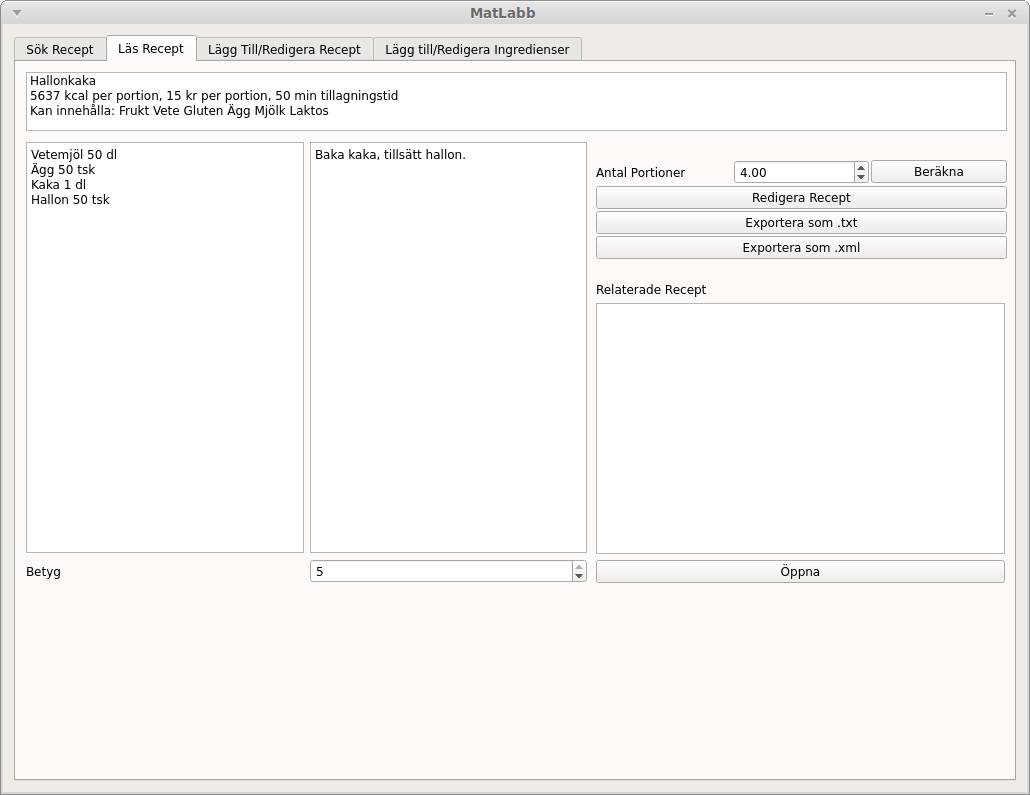
\includegraphics[scale=0.44]{las_recept.png} 
        \caption{Läs receptvyn} 
        \label{fig:receptvyn}
\end{figure}

I \verb+Läs recept+-vyn möts man av ett flertal fält. I huvudfältet längst upp finner
man information om receptets namn, energimängd per portion,
ingrediensernas summerade kostnad per portion och hur lång tid receptet tar att laga till. Finns det allergener i någon av receptets ingredienser så skrivs även det ut.

Under huvudfönstret finns från vänster sett Ingrediensfältet,
instruktionsfältet samt portionsskalning och knappar för export
och redigering. I ingrediensfältet finns de ingredienser som krävs
samt behövd mängd. I instruktionsfältet finner man de instruktioner som krävs för att följa det öppna receptet. 

Till höger om instruktionsfältet finns portionsskalaren. Med pilarna eller tangentbordet kan antalet portioner ändras och när knappen \verb+beräkna+ trycks in
skalas mängden ingredienser i ingrediensfältet om. Under knapparna för redigering och export finns en
lista över relaterade recept. Man kan klicka på titeln hos ett relaterat recept och sedan på knappen \verb+öppna+. Man stannar då kvar i receptvyn, men informationen i varje fält byts ut mot respektive hos det nyöppnade receptet. 

Nederst i fönstret kan receptets betyg redigeras med pilarna eller genom att mata in en siffra från ett till fem med tangentbordet.

Knappen \verb+Redigera Recept+ används för att öppna receptet för redigering. Finns det ett öppet recept när denna beklickas skickas man till vyn Lägg till/Uppdatera recept. Vyn förklaras ingående i nästa kapitel.
